\chapter{Fazit}
\label{chap:Fazit}
Ziel dieser Arbeit war es, die Gemeinsamkeiten und Unterschiede zwischen SOA und Microservices herauszuarbeiten. Dazu wurden die Vor- und Nachteile der beiden Paradigmen hinsichtlich Prozessisolierung, Skalierung, Deployment, Wartbarkeit (Korrigierbarkeit, Erweiterbarkeit, Anpassbarkeit, Verbesserung), Entwicklung/Testbarkeit und die Bindung an Technologiestacks herausgearbeitet und anschließend verglichen werden.
\\\\
Nach der Analyse und dem Vergleich der beiden Paradigmen, kann man sagen, dass beide Paradigmen, unterschiedliche Ansätze verfolgen. Während bei dem Microservice Paradigma, eine Anwendung in kleinere Dienste, sogenannte Microservices, aufgeteilt wird, um die Entwicklung zu vereinfachen. Das SOA Paradigma hingegen verwendet vollständige Anwendungen, in Kombination eines dafür entwickelten Adapters, als Dienst. SOA soll die Kommunikation zwischen den einzelnen Anwendungen standardisieren und aufbereiten. Dabei soll darauf geachtet werden, dass die Benutzer der Dienste, nur die Informationen bereitgestellt bekommen, welche sie wirklich benötigen. In einem Unternehmen existiert nur ein einziges SOA-System, es können jedoch mehrere Microservice-Systeme vorhanden sein.
\\\\
SOA und Microservices schließen sich nicht gegenseitig aus. Microservice-Systeme können Teil eines SOA-Systems sein und ihre Aufgaben in diesen einbinden. Dabei wird ein Microservice-System wie eine vollständige Anwendung behandelt. Der  Unterschied ist jedoch, dass meistens deutlich mehr Schnittstellen zur Verfügung gestellt werden können, aufgrund der internen Struktur.
\begin{figure}[htb]
    \centering 
    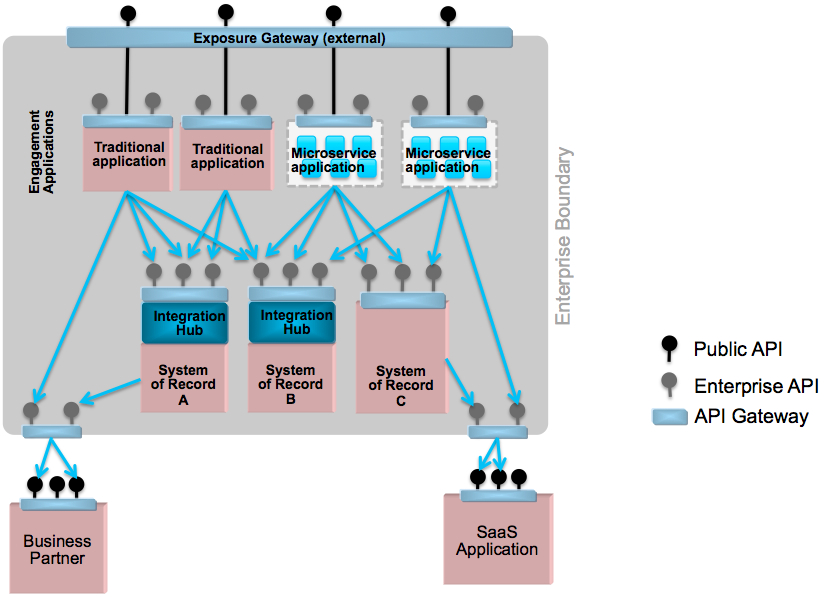
\includegraphics[width=\textwidth]{content/images/figure8}\
    \quelle\url{https://www.ibm.com/developerworks/websphere/library/techarticles/1601_clark-trs/1601_clark.html}
    \caption{Microservice, SOA und APIs Kombiniert}
    \label{fig:MicroservicesSOAAndAPIsCombined} 
\end{figure}

Möchte man eine Service-orientierte Architektur einsetzten, muss zunächst einmal die Frage gestellt werden, welchen Zweck damit erfüllt werden soll. Möchte man den Softwareentwicklungsprozess eines Unternehmens unterstützen, so sollte das Microservice Paradigma, vor dem SOA Paradigma  gewählt werden. Möchte man jedoch die Businessprozesse in einem Unternehmen verbessern, sollte das SOA Paradigma eingesetzt werden.
\\\\
Es sollte jedoch nicht nur die Fragen nach dem Zweck gestellt werden, sondern auch nach den Einsatzmöglichkeiten. Wird ein System benötigt, welches einfach zu skalieren ist oder ein System, bei dem der Benutzer nur die Informationen zur Verfügung gestellt bekommt, welche wirklich benötigt werden. Während in einem Microservice-System deutlich einfacher Skaliert werden kann, als in einem SOA-System, werden durch die Schnittstellen sehr viele Informationen bereitgestellt. Bei einem SOA-System hingegen wird dafür gesorgt, dass die Informationen gefiltert und aufbereitet werden, sodass der Nutzer nur die Informationen bekommt, welche er benötigt, jedoch kann nicht schnell skaliert werden.
\\\\
Es muss dementsprechend gut überlegt werden, welches Paradigma eingesetzt werden soll. Zudem sollte man sich den Aufwand bewusstwerden, welcher benötigt wird, um das eingesetzte Paradigma einzusetzen.

\section{Ausblick}
\label{sec:Ausblick}
In der Bachelorarbeit soll eine Anwendung, für die Zusammenarbeit, beispielhaft mit dem Microservice Paradigma erstellt werden. Anhand diesem beispielhaften System soll untersucht werden, welche Voraussetzungen gegeben sein müssen, um ein Microservice-System zu betreiben und welche Werkzeuge eingesetzt werden müssen, um ein Microservice-System aufzubauen, bzw. zu verwenden und zu verwalten. Konkret soll Untersucht werden, wie genau ein Microservice deployed und skaliert werden kann. Zudem soll untersucht werden wie Microservices in solch einem System gefunden und verwendet werden können. außerdem soll untersucht werden, wie die Benutzerverwaltung und die Authentifizierung in solch einem System funktioniert. Konkret soll untersucht werden, wie Benutzerberechtigungen verwaltet und abgefragt werden können, welche unterschiedlichen Ansätze dafür existieren und welche Vor- und Nachteile die jeweiligen Ansätze besitzen. Zusätzlich soll untersucht werden, wie das Monitoring in solch einem System funktioniert.